
\documentclass[12pt]{article}

% Layout.
\usepackage[top=1in, bottom=0.75in, left=1in, right=1in, headheight=1in, headsep=6pt]{geometry}

% Fonts.
\usepackage{mathptmx}
\usepackage[scaled=0.86]{helvet}
\renewcommand{\emph}[1]{\textsf{\textbf{#1}}}

% TiKZ.
\usepackage{tikz, pgfplots,mathrsfs}
\usetikzlibrary{calc}
\pgfplotsset{compat = newest}
 
\pgfplotsset{my style/.append style={axis x line=middle, axis y line=
middle, xlabel={$x$}, ylabel={$y$}, axis equal
}}

% Misc packages.
\usepackage{amsmath,amssymb,latexsym}
\usepackage{graphicx}
\usepackage{array}
\usepackage{xcolor}
\usepackage{multicol}

% Commands to set various header/footer components.
\makeatletter
\def\doctitle#1{\gdef\@doctitle{#1}}
\doctitle{Use {\tt\textbackslash doctitle\{MY LABEL\}}.}
\def\docdate#1{\gdef\@docdate{#1}}
\docdate{Use {\tt\textbackslash docdate\{MY DATE\}}.}
\def\doccourse#1{\gdef\@doccourse{#1}}
\let\@doccourse\@empty
\def\docscoring#1{\gdef\@docscoring{#1}}
\let\@docscoring\@empty
\def\docversion#1{\gdef\@docversion{#1}}
\let\@docversion\@empty
\makeatother

% Headers and footers layout.
\makeatletter
\usepackage{fancyhdr}
\pagestyle{fancy}
\fancyhf{} % Clears all headers/footers.
\lhead{\baselineskip 30pt
%\emph{\@doctitle\hfill\@docdate}
\emph{\@docdate\hfill\@doctitle}
\ifnum \value{page} > 1\relax\else\\
\emph{Name: \rule{3.5in}{1pt}\hfill \@docscoring}\fi}
\rfoot{\emph{\@docversion}}
\lfoot{\emph{\@doccourse}}
\cfoot{\emph{\thepage}}
\renewcommand{\headrulewidth}{0pt}%
\makeatother

% Paragraph spacing
\parindent 0pt
\parskip 6pt plus 1pt

% A problem is a section-like command. Use \problem{5} to
% start a problem worth 5 points.
\newcounter{probcount}
\newcounter{subprobcount}
\setcounter{probcount}{0}
\newcommand{\problem}[1]{%
\par
\addvspace{4pt}%
\setcounter{subprobcount}{0}%
\stepcounter{probcount}%
\makebox[0pt][r]{\emph{\arabic{probcount}.}\hskip1ex}\emph{[#1 points]}\hskip1ex}
\newcommand{\thesubproblem}{\emph{\alph{subprobcount}.}}

% Subproblems are an enumerate-like environment with a consistent
% numbering scheme. 
% Use \begin{subproblems}\item...\item...\end{subproblems}
\newenvironment{subproblems}{%
\begin{enumerate}%
\setcounter{enumi}{\value{subprobcount}}%
\renewcommand{\theenumi}{\emph{\alph{enumi}}}}%
{\setcounter{subprobcount}{\value{enumi}}\end{enumerate}}

% Blanks for answers in normal and math mode.
\newcommand{\blank}[1]{\rule{#1}{0.75pt}}
\newcommand{\mblank}[1]{\underline{\hspace{#1}}}
\def\emptybox(#1,#2){\framebox{\parbox[c][#2]{#1}{\rule{0pt}{0pt}}}}

% Misc.
\renewcommand{\d}{\displaystyle}
\newcommand{\ds}{\displaystyle}
\def\bc{\begin{center}}
\def\ec{\end{center}}
\def\be{\begin{enumerate}}
\def\ee{\end{enumerate}}


\doctitle{Math F251X: Quiz 10}
\docdate{December 3, 2023}
\doccourse{UAF Calculus I}
\docversion{v-1 async}
\docscoring{\blank{0.8in} / 25}
\begin{document}
%\textbf{Please circle your instructor's name:} \hfill Leah Berman  \hfill   Jill Faudree\\

There are 25 points possible on this quiz.  {\it You should be able to complete it without using your notes or textbook or a calculator --- this is practice for your exams!} If you needed to look something up, you should to me about questions you might have.  {\bf Show all work for full credit} and use some words or sentences to help communicate your answers.

% area so far functions
\problem{4} Define $\displaystyle{G(x)=\int_0^x f(t) \ dt}$ where the graph of $f(t)$ is drawn below.\\
\begin{minipage}{.5\textwidth}
\begin{center}
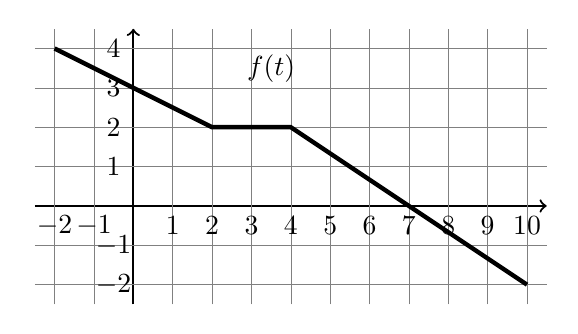
\begin{tikzpicture}[scale=.5]
\draw[thick, ->] (0,-2.5) -- (0,4.5);
\draw[thick, ->] (-2.5,0) -- (10.5,0);
\foreach \i in {-2,-1,1,2,3,4}{
	\draw[help lines] (-2.5,\i) -- (10.5,\i);
	\draw[help lines] (\i,-2.5) -- (\i,4.5);
	\node at (\i, -0.5){$\i$};
	\node at (-0.5,\i){$\i$};
	}
\foreach \i in {5,6,7,8,9,10}{
	%\draw[dashed] (-2.5,\i) -- (8.5,\i);
	\draw[help lines] (\i,-2.5) -- (\i,4.5);
	\node at (\i, -0.5){$\i$};
	%\node at (-0.5,\i){$\i$};
	}

%\draw (-.5,5) -- (0.5,5);
%\node at (-1,5.2){5};
\draw[ultra thick] (-2,4)--(2,2) -- (4,2) -- (10,-2);
\node at (3.5,3.5){$f(t)$};
%\draw[black, line width = 0.40mm, dashed]   plot[smooth,domain=-4.2:4.2] (\x, {5-0.333*\x*\x});
\end{tikzpicture}
\end{center}
\end{minipage}
\begin{minipage}{.5\textwidth}
	\begin{subproblems}
	\item Determine $G(4).$ 
	\vspace{.5in}
	\item Does $G(x)$ have a maximum on the interval $[0,10]$? Explain your answer.
		\vspace{.75in}
	\end{subproblems}
\end{minipage}
%FTC part 2
\problem{6} Evaluate each definite integral using the Fundamental Theorem of Calculus Part 2.
	\begin{subproblems}
	\item $\displaystyle \int_1^{9} \frac{6}{\sqrt{x}} \: dx$
	\vfill
	\item $\displaystyle \int_{0}^{\pi/3} (12-2\sin(x)) \: dx$
	\vfill
	\end{subproblems}
	
	
\problem{4} Evaluate $\ds \int_{0}^{\pi/4} (\sec(\theta))^{2} \tan(\theta) \: d\theta$. Show your work.

\vfill
	
	\newpage

%FTC part 1
\problem{6} Use the Fundamental Theorem of Calculus (Part 1) to find each derivative.
	\begin{subproblems}
	\item $\displaystyle \frac{d}{dx} \left( \int_6^x t^{5} - \frac{2}{t} \: dt \right)$
	\vfill
	\item $\displaystyle \frac{d}{dx} \left( \int_{\cos(x)}^4 \sqrt{1-t^2} \: dt \right)$
	\vfill
	\end{subproblems}


	
% substitution!



\problem{5} A ball is thrown upward from an initial height of $4$ ft at an initial speed of $10$ ft/s. The acceleration due to gravity is $32$ ft/s$^2$. (Just to be clear, we are assuming $a(t)=-32$ is the equation modeling the acceleration of the ball.)\\
	\begin{subproblems}
	\item Solve for $v(t)$, the velocity of the ball $t$ seconds after it is thrown into the air. (Use calculus techniques.)\\
	\vfill 
	\item Solve for $h(t)$, the height of the ball $t$ seconds after it is thrown into the air. (Use calculus techniques.)\\
	\vfill 
	\item At what time is the ball the highest? Show your work, and answer the question with a sentence.
	\vfill
	\end{subproblems} 

%\problem{6} The function $f(t)$ measures the rate of water usage in a household over a 24 hour period, where $f$ is measured in gallons per hour and $t$ is measured in hours starting at 12:00 am. (So, at 12 midnight, $t=0$). Write a complete sentence in clear English (not calculus), including units, explaining the meaning of each quantity below. \begin{subproblems}
%	\item $f(7)=126$\\ %note: 2.1 gallons/minute is average flow rate
%	\vfill
%	\item $\displaystyle{\int_{6.5}^{7.5} f(t) \: dt = 17.2}$ % apparently the average shower lasts 8.2 minutes and uses 17.2 gallons of water. Only one shower in this household in the morning, apparently.
%	\vfill
%\end{subproblems}
	

\end{document}
